\documentclass[]{elsarticle} %review=doublespace preprint=single 5p=2 column
%%% Begin My package additions %%%%%%%%%%%%%%%%%%%
\usepackage[hyphens]{url}
\usepackage{lineno} % add
\providecommand{\tightlist}{%
  \setlength{\itemsep}{0pt}\setlength{\parskip}{0pt}}

\bibliographystyle{elsarticle-harv}
\biboptions{sort&compress} % For natbib
\usepackage{graphicx}
\usepackage{booktabs} % book-quality tables
%% Redefines the elsarticle footer
%\makeatletter
%\def\ps@pprintTitle{%
% \let\@oddhead\@empty
% \let\@evenhead\@empty
% \def\@oddfoot{\it \hfill\today}%
% \let\@evenfoot\@oddfoot}
%\makeatother

% A modified page layout
\textwidth 6.75in
\oddsidemargin -0.15in
\evensidemargin -0.15in
\textheight 9in
\topmargin -0.5in
%%%%%%%%%%%%%%%% end my additions to header

\usepackage[T1]{fontenc}
\usepackage{lmodern}
\usepackage{amssymb,amsmath}
\usepackage{ifxetex,ifluatex}
\usepackage{fixltx2e} % provides \textsubscript
% use upquote if available, for straight quotes in verbatim environments
\IfFileExists{upquote.sty}{\usepackage{upquote}}{}
\ifnum 0\ifxetex 1\fi\ifluatex 1\fi=0 % if pdftex
  \usepackage[utf8]{inputenc}
\else % if luatex or xelatex
  \usepackage{fontspec}
  \ifxetex
    \usepackage{xltxtra,xunicode}
  \fi
  \defaultfontfeatures{Mapping=tex-text,Scale=MatchLowercase}
  \newcommand{\euro}{€}
\fi
% use microtype if available
\IfFileExists{microtype.sty}{\usepackage{microtype}}{}
\usepackage{longtable}
\usepackage{graphicx}
% We will generate all images so they have a width \maxwidth. This means
% that they will get their normal width if they fit onto the page, but
% are scaled down if they would overflow the margins.
\makeatletter
\def\maxwidth{\ifdim\Gin@nat@width>\linewidth\linewidth
\else\Gin@nat@width\fi}
\makeatother
\let\Oldincludegraphics\includegraphics
\renewcommand{\includegraphics}[1]{\Oldincludegraphics[width=\maxwidth]{#1}}
\ifxetex
  \usepackage[setpagesize=false, % page size defined by xetex
              unicode=false, % unicode breaks when used with xetex
              xetex]{hyperref}
\else
  \usepackage[unicode=true]{hyperref}
\fi
\hypersetup{breaklinks=true,
            bookmarks=true,
            pdfauthor={},
            pdftitle={The genome of Pocillopora damicornis and comparative genomics of scleractinian corals},
            colorlinks=true,
            urlcolor=blue,
            linkcolor=magenta,
            pdfborder={0 0 0}}
\urlstyle{same}  % don't use monospace font for urls
\setlength{\parindent}{0pt}
\setlength{\parskip}{6pt plus 2pt minus 1pt}
\setlength{\emergencystretch}{3em}  % prevent overfull lines
\setcounter{secnumdepth}{0}
\usepackage{lineno}
\linenumbers
% Pandoc toggle for numbering sections (defaults to be off)
\setcounter{secnumdepth}{0}
% Pandoc header
\usepackage{lineno}
\linenumbers


\usepackage[nomarkers]{endfloat}

\begin{document}
\begin{frontmatter}

  \title{The genome of \emph{Pocillopora damicornis} and comparative genomics of
scleractinian corals}
    \author[RSMAS]{Ross Cunning\corref{c1}}
   \ead{ross.cunning@gmail.com} 
   \cortext[c1]{Corresponding Author}
    \author[UCLA]{Rachael A. Bay}
  
  
    \author[RSMAS]{Andrew C. Baker}
  
  
    \author[RSMAS]{Nikki Traylor-Knowles}
  
  
      \address[RSMAS]{Department of Marine Biology and Ecology, Rosenstiel School of Marine
and Atmospheric Science, University of Miami, Miami, FL 33149, USA}
    \address[UCLA]{Institute for the Environment and Sustainability, University of
California, Los Angeles, Los Angeles, CA 90095, USA}
  
  \begin{abstract}
  Abstract text here.
  \end{abstract}
  
 \end{frontmatter}

\section{Abstract}\label{abstract}

\section{Introduction}\label{introduction}

Scleractinian corals serve the critical ecological role of building
reefs that provide billions of dollars annually in goods and services
(Costanza, Groot, and Sutton 2014) and sustain high levels of
biodiversity (Knowlton et al. 2010). Moreover, as basal metazoans,
corals provide a model for studying the evolution of key traits such as
symbiosis (Neubauer et al. 2016), immunity (Quistad et al. 2014), and
biomineralization (Takeuchi et al. 2016). However, corals are declining
rapidly due to ocean acidification, which impairs coral skeleton
formation (Kleypas et al. 1999), and ocean warming, which disrupts their
symbiosis with photosynthetic \emph{Symbiodinium} spp. (Jokiel and Coles
1977). Understanding the genomic architecture of these traits and their
responses to climate change is therefore key to understanding corals'
success through evolutionary history (Bhattacharya et al. 2016) and in
future climate scenarios. In particular, there is great interest in
whether corals possess the genetic basis and genetic variation required
to acclimatize and/or adapt to rapid climate change (Oppen et al. 2015;
Dixon et al. 2015; R. A. Bay et al. 2017). Addressing these questions
requires expanding genomic resources for corals, and establishes a
fundamental role for comparative genomic analysis in these organisms.

Genomic resources for corals have expanded rapidly in recent years, with
genomic or transcriptomic information available for at least 20 coral
species (see Bhattacharya et al. (2016)). Comparative analysis of these
data has identified genes that may be important in biomineralization,
symbiosis, and environmental stress responses (Bhattacharya et al.
2016). However, complete genome sequences have only been analyzed and
compared for two coral species, \emph{Acropora digitifera} and
\emph{Stylophora pistillata} (Voolstra et al. 2017), which revealed
extensive differences in genomic architecture and content. Therefore,
additional complete coral genomes and more comprehensive comparative
analysis may be transformative in our understanding of the genomic
content and evolutionary history of reef-building corals.

Here, we present the genome of \emph{Pocillopora damicornis}, one of the
most abundant and widespread reef-building corals in the Indo-Pacific.
This ecologically important coral is the subject of a large body of
research on speciation (J. H. Pinzón et al. 2013; Schmidt-Roach et al.
2014; Johnston et al. 2017), population genetics (J. a Stoddart 1984; J.
H. Pinzón and LaJeunesse 2011; Combosch and Vollmer 2011; L. Thomas et
al. 2017), symbiosis ecology (Glynn et al. 2001; McGinley et al. 2012;
Cunning and Baker 2013), and reproduction (J. A. Stoddart 1983; Ward
1992; Schmidt-Roach et al. 2012), and is commonly used in experimental
biology and physiology. Therefore, availability of the \emph{P.
damicornis} genome will advance a number of fields in coral biology,
ecology, and evolution, and provides a direct foundation for future
studies in transcriptomics, population genomics, and functional
genomics.

Using this genome and other publicly available genomes of corals,
Cnidarians, and basal metazoans, we provide the most comprehensive
comparative genomic analysis to date in Scleractinia. In particular, we
address critical questions such as: 1) what constitutes the `core
genome' common to all corals, 2) what genes are specific to or
diversified within corals, and 3) what genes are specific to or
diversified within individual coral species, providing insight into the
evolution of Scleractinia.

\section{Materials and Methods}\label{materials-and-methods}

\subsection{\texorpdfstring{\emph{P. damicornis} genome sequencing and
assembly}{P. damicornis genome sequencing and assembly}}\label{p.-damicornis-genome-sequencing-and-assembly}

The \emph{P. damicornis} genotype used for sequencing was collected at
Isla de Saboga, Panama in March 2005, and cultured indoors at the
University of Miami Coral Resource Facility until the time of sampling.
Genomic DNA was extracted from two fragments of this genotype in XXX
2016 using XXX protocol. DNA was delivered to Dovetail Genomics (Santa
Cruz, CA, USA), where Chicago libraries were prepared and sequenced on
an Illumina XXX platform, and genome scaffolds were assembled \emph{de
novo} using the HiRise software pipeline (N. H. Putnam et al. 2016). The
Dovetail HiRise scaffolds were then filtered to remove those of
potential non-coral origin using BLAST (Altschul et al. 1990) searches
against three databases: 1) \emph{Symbiodinium}, containing the genomes
of \emph{S. minutum} (Shoguchi et al. 2013) and \emph{S.
microadriaticum} (M. Aranda et al. 2016), 2) bacteria, containing 6954
complete bacterial genomes from NCBI, and 3) viruses, containing 2996
viral genomes from the phantome database (phantome.org; accessed
2017-03-01). Scaffolds with a BLAST hit to any of these databases with
an e-value \textless{} 10\textsuperscript{-20} and a bitscore
\textgreater{} 1000 were considered to be non-coral in origin and
removed from the assembly (Baumgarten et al. 2015).

\subsection{\texorpdfstring{\emph{P. damicornis} genome
annotation}{P. damicornis genome annotation}}\label{p.-damicornis-genome-annotation}

The filtered assembly was analyzed for completeness using BUSCO (Simão
et al. 2015) to search for 978 universal metazoan single-copy orthologs.
The \texttt{-\/-long} option was passed to BUSCO in order to train the
\emph{ab initio} gene prediction software Augustus (M. Stanke et al.
2004). Augustus gene prediction parameters were then used in the MAKER
pipeline (Campbell et al. 2014) to annotate gene models, using as
supporting evidence two RNA-seq datasets from \emph{P. damicornis}
{[}Mayfield?; Traylor-Knowles/Bhattacharya?{]} and one from
closely-related \emph{Stylophora pistillata} (Voolstra et al. 2017), and
protein sequences from 20 coral species (Bhattacharya et al. 2016).
Results from this initial MAKER run were used to train a second gene
predictor (SNAP ({\textbf{???}})) prior to an iterative MAKER run to
refine gene models. Predicted protein sequences were then extracted from
the assembly and putative functional annotations were added by searching
for homologous proteins in the Uniprot-Swissprot database
(The~UniProt~Consortium 2017) using BLAST
(E\textless{}10\textsuperscript{-5}), and protein domains using
InterProScan (Finn et al. 2017). Genome annotation summary statistics
were generated using the Genome Annotation Generator software (Hall,
DeRego, and Geib 2014).

\subsection{Comparative genomic
analyses}\label{comparative-genomic-analyses}

We identified ortholog groups (gene families) among the predicted
proteins of four scleractinians, two corallimorpharians, two anemones,
one hydrozoan, one sponge, and one ctenophore (Table 1) using the
software fastOrtho (http://enews.patricbrc.org/fastortho/) based on the
MCL algorithm with a blastp E-value cutoff of 10\textsuperscript{-5}.
Based on these orthologous gene families, we defined and extracted
several gene sets of interest: 1) gene families that were shared by all
four corals (i.e., coral `core' genes), 2) genes that were present in
all four corals but absent from other organisms (i.e., coral-specific
genes), 3) gene families that were significantly larger in corals
relative to other anthozoans (Binomial generalized linear model,
FDR-adjusted \emph{p}\textless{}0.01; i.e., coral-diversified genes), 4)
gene families that were significantly larger in a single coral species
relative to all other corals (pairwise comparisons using Fisher's exact
test, FDR-adjusted \emph{p}\textless{}0.01; i.e., coral species-specific
gene family expansions), and 5) genes present in \emph{P. damicornis}
with no orthologs in any other genome (i.e., \emph{P.
damicornis}-specific genes).

\subsection{Functional
characterization}\label{functional-characterization}

Putative gene functionality was characterized using Gene Ontology (GO)
analysis. GO terms were assigned to predicted \emph{P. damicornis}
protein sequences using InterProScan (Jones et al. 2014). Significantly
enriched GO terms in gene sets of interest relative to the whole genome
were identified using the R package topGO (Alexa and Rahnenfuhrer 2016),
and significantly enriched GO terms were clustered and visualized using
REVIGO (Supek et al. 2011). These analyses were implemented using custom
scripts in R, Python, and Unix shell, which are available in the
accompanying data repository (github.com/jrcunning/pdam-genome).

\section{Results and discussion}\label{results-and-discussion}

\subsection{Genome assembly and annotation
statistics}\label{genome-assembly-and-annotation-statistics}

The estimated true genome size of \emph{P. damicornis} is 348 Mb,
smaller than other coral genomes analyzed to date. The size of the final
assembly produced here was 234 Mb, and likely lacks high-identity repeat
content that could not be assembled. The assembly comprises 96.3\%
contiguous sequence, and has the highest contig N50 (28.5 kb) of any
cnidarian genome assembly (Table 1). We identified 26077 gene models,
with 21389 (82\%) of these being apparently complete with start and stop
codons. This number of genes is very close to the average reported in
other scleractinian and cnidarian genomes (Table 1). Of these 26077 gene
models, 59.7 had identifiable homologs (E-value \(\leq\)
10\textsuperscript{-5}) in the UniProt-SwissProt database, and 83.7
contained protein domains annotated by InterProScan. In addition, 73\%
of genes contained identifiable homologs in at least one of the other 10
genomes analyzed here. Furthermore, out of 978 metazoan single-copy
orthologs, a BUSCO search found that 865 (88.4\%) of these were present
and complete (5 of these were duplicated). An additional 28 orthologs
were present but fragmented, and 85 (8.7\%) were missing. Together,
these statistics indicate the \emph{P. damicornis} genome assembly is
the highest quality and most complete scleractinian genome to date
(Table 1).

\begin{table}[H]
\centering
\resizebox{\linewidth}{!}{\begin{tabular}{llllllllllll}
\toprule
  & Pdam & Spis & Adig & Ofav & Disc & Afen & Aipt & Nema & Hydr & Mlei & Aque\\
\midrule
Genome size (Mb) & 348 & 434 & 420 &  & 428 & 350 & 260 & 329 & 1300 &  & 190\\
Assembly size (Mb) & 234 & 400 & 419 & 486 & 445 & 370 & 258 & 356 & 852 & 156 & 167\\
Total contig size (Mb) & 226 & 358 & 365 & 356 & 364 & 306 & 213 & 297 & 785 & 150 & 145\\
Contig / Assemly (\%) & 96.3 & 89.5 & 87 & 73.3 & 81.9 & 82.6 & 82.5 & 83.4 & 92.2 & 96.5 & 86.8\\
Contig N50 (kb) & 25.9 & 14.9 & 10.9 & 7.4 & 18.7 & 20.1 & 14.9 & 19.8 & 9.7 & 11.9 & 11.2\\
\addlinespace
Scaffold N50 (kb) & 326 & 457 & 191 & 1162 & 770 & 510 & 440 & 472 & 92.5 & 187 & 120\\
No. gene models & 26077 & 25769 & 23668 & 37660 & 23199 & 21372 & 29269 & 27273 & 31452 & 16554 & 29867\\
No. complete gene models & 21389 & 25563 & 16434 & 29679 & 16082 & 15552 & 26658 & 13343 &  &  & \\
BUSCO completeness (\%) & 88.4 & 72.2 & 34.3 & 71 &  &  &  &  &  &  & \\
Mean exon length (bp) & 245 & 262 & 230 & 240 & 226 & 218 & 354 & 208 &  & 314 & \\
\addlinespace
Mean intron length (bp) & 667 & 917 & 952 & 1146 & 1119 & 1047 & 638 & 800 &  & 898 & 80\\
Mean protein length (aa) & 455 & 615 & 424 & 413 & 450 & 475 & 517 & 331 &  & 154? & 280(med)\\
\bottomrule
\multicolumn{12}{l}{\textsuperscript{*} table footnote}\\
\end{tabular}}
\end{table}

\begin{longtable}[]{@{}llllllllllll@{}}
\caption{Assembly and annotation statistics for the \emph{P. damicornis}
genome (Pdam) and others used for comparative analysis.
(Spis=\emph{Stylophora pistillata} (Voolstra et al. 2017);
Adig=\emph{Acropora digitifera} (Shinzato et al. 2011);
Ofav=\emph{Orbicella faveolata} (Prada et al. 2016);
Disc=\emph{Discosoma spp.} (Wang et al. 2017); Afen=\emph{Amplexidiscus
fenestrafer} (Wang et al. 2017); Aipt=\emph{Aiptasia} (Baumgarten et al.
2015); Nema=\emph{Nematostella vectensis} (N. H. Putnam et al. 2007);
Hydr=\emph{Hydra vulgaris} (J. a Chapman et al. 2010);
Mlei=\emph{Mnemiopsis leidyi} (J. F. Ryan et al. 2013);
Aque=\emph{Amphimedon queenslandica} (Srivastava et al.
2010)).}\tabularnewline
\toprule
\begin{minipage}[b]{0.15\columnwidth}\raggedright\strut
\strut
\end{minipage} & \begin{minipage}[b]{0.05\columnwidth}\raggedright\strut
Pdam\strut
\end{minipage} & \begin{minipage}[b]{0.05\columnwidth}\raggedright\strut
Spis\strut
\end{minipage} & \begin{minipage}[b]{0.05\columnwidth}\raggedright\strut
Adig\strut
\end{minipage} & \begin{minipage}[b]{0.05\columnwidth}\raggedright\strut
Ofav\strut
\end{minipage} & \begin{minipage}[b]{0.05\columnwidth}\raggedright\strut
Disc\strut
\end{minipage} & \begin{minipage}[b]{0.05\columnwidth}\raggedright\strut
Afen\strut
\end{minipage} & \begin{minipage}[b]{0.05\columnwidth}\raggedright\strut
Aipt\strut
\end{minipage} & \begin{minipage}[b]{0.05\columnwidth}\raggedright\strut
Nema\strut
\end{minipage} & \begin{minipage}[b]{0.05\columnwidth}\raggedright\strut
Hydr\strut
\end{minipage} & \begin{minipage}[b]{0.05\columnwidth}\raggedright\strut
Mlei\strut
\end{minipage} & \begin{minipage}[b]{0.05\columnwidth}\raggedright\strut
Aque\strut
\end{minipage}\tabularnewline
\midrule
\endfirsthead
\toprule
\begin{minipage}[b]{0.15\columnwidth}\raggedright\strut
\strut
\end{minipage} & \begin{minipage}[b]{0.05\columnwidth}\raggedright\strut
Pdam\strut
\end{minipage} & \begin{minipage}[b]{0.05\columnwidth}\raggedright\strut
Spis\strut
\end{minipage} & \begin{minipage}[b]{0.05\columnwidth}\raggedright\strut
Adig\strut
\end{minipage} & \begin{minipage}[b]{0.05\columnwidth}\raggedright\strut
Ofav\strut
\end{minipage} & \begin{minipage}[b]{0.05\columnwidth}\raggedright\strut
Disc\strut
\end{minipage} & \begin{minipage}[b]{0.05\columnwidth}\raggedright\strut
Afen\strut
\end{minipage} & \begin{minipage}[b]{0.05\columnwidth}\raggedright\strut
Aipt\strut
\end{minipage} & \begin{minipage}[b]{0.05\columnwidth}\raggedright\strut
Nema\strut
\end{minipage} & \begin{minipage}[b]{0.05\columnwidth}\raggedright\strut
Hydr\strut
\end{minipage} & \begin{minipage}[b]{0.05\columnwidth}\raggedright\strut
Mlei\strut
\end{minipage} & \begin{minipage}[b]{0.05\columnwidth}\raggedright\strut
Aque\strut
\end{minipage}\tabularnewline
\midrule
\endhead
\begin{minipage}[t]{0.15\columnwidth}\raggedright\strut
Genome size (Mb)\strut
\end{minipage} & \begin{minipage}[t]{0.05\columnwidth}\raggedright\strut
348\textsuperscript{\$}\strut
\end{minipage} & \begin{minipage}[t]{0.05\columnwidth}\raggedright\strut
434\strut
\end{minipage} & \begin{minipage}[t]{0.05\columnwidth}\raggedright\strut
420\strut
\end{minipage} & \begin{minipage}[t]{0.05\columnwidth}\raggedright\strut
\strut
\end{minipage} & \begin{minipage}[t]{0.05\columnwidth}\raggedright\strut
428\strut
\end{minipage} & \begin{minipage}[t]{0.05\columnwidth}\raggedright\strut
350\strut
\end{minipage} & \begin{minipage}[t]{0.05\columnwidth}\raggedright\strut
260\strut
\end{minipage} & \begin{minipage}[t]{0.05\columnwidth}\raggedright\strut
329{[}\^{}e{]}\strut
\end{minipage} & \begin{minipage}[t]{0.05\columnwidth}\raggedright\strut
1300\strut
\end{minipage} & \begin{minipage}[t]{0.05\columnwidth}\raggedright\strut
\strut
\end{minipage} & \begin{minipage}[t]{0.05\columnwidth}\raggedright\strut
190\strut
\end{minipage}\tabularnewline
\begin{minipage}[t]{0.15\columnwidth}\raggedright\strut
Assembly size (Mb)\strut
\end{minipage} & \begin{minipage}[t]{0.05\columnwidth}\raggedright\strut
234\strut
\end{minipage} & \begin{minipage}[t]{0.05\columnwidth}\raggedright\strut
400\strut
\end{minipage} & \begin{minipage}[t]{0.05\columnwidth}\raggedright\strut
419\strut
\end{minipage} & \begin{minipage}[t]{0.05\columnwidth}\raggedright\strut
486\strut
\end{minipage} & \begin{minipage}[t]{0.05\columnwidth}\raggedright\strut
445\strut
\end{minipage} & \begin{minipage}[t]{0.05\columnwidth}\raggedright\strut
370\strut
\end{minipage} & \begin{minipage}[t]{0.05\columnwidth}\raggedright\strut
258\strut
\end{minipage} & \begin{minipage}[t]{0.05\columnwidth}\raggedright\strut
356\strut
\end{minipage} & \begin{minipage}[t]{0.05\columnwidth}\raggedright\strut
852\strut
\end{minipage} & \begin{minipage}[t]{0.05\columnwidth}\raggedright\strut
156\strut
\end{minipage} & \begin{minipage}[t]{0.05\columnwidth}\raggedright\strut
167\strut
\end{minipage}\tabularnewline
\begin{minipage}[t]{0.15\columnwidth}\raggedright\strut
Total contig size (Mb)\strut
\end{minipage} & \begin{minipage}[t]{0.05\columnwidth}\raggedright\strut
226\strut
\end{minipage} & \begin{minipage}[t]{0.05\columnwidth}\raggedright\strut
358\strut
\end{minipage} & \begin{minipage}[t]{0.05\columnwidth}\raggedright\strut
365\strut
\end{minipage} & \begin{minipage}[t]{0.05\columnwidth}\raggedright\strut
356\strut
\end{minipage} & \begin{minipage}[t]{0.05\columnwidth}\raggedright\strut
364\strut
\end{minipage} & \begin{minipage}[t]{0.05\columnwidth}\raggedright\strut
306\strut
\end{minipage} & \begin{minipage}[t]{0.05\columnwidth}\raggedright\strut
213\strut
\end{minipage} & \begin{minipage}[t]{0.05\columnwidth}\raggedright\strut
297\strut
\end{minipage} & \begin{minipage}[t]{0.05\columnwidth}\raggedright\strut
785\strut
\end{minipage} & \begin{minipage}[t]{0.05\columnwidth}\raggedright\strut
150\strut
\end{minipage} & \begin{minipage}[t]{0.05\columnwidth}\raggedright\strut
145\strut
\end{minipage}\tabularnewline
\begin{minipage}[t]{0.15\columnwidth}\raggedright\strut
Contig / Assembly (\%)\strut
\end{minipage} & \begin{minipage}[t]{0.05\columnwidth}\raggedright\strut
96.3\strut
\end{minipage} & \begin{minipage}[t]{0.05\columnwidth}\raggedright\strut
89.5\strut
\end{minipage} & \begin{minipage}[t]{0.05\columnwidth}\raggedright\strut
87.0\strut
\end{minipage} & \begin{minipage}[t]{0.05\columnwidth}\raggedright\strut
73.3\strut
\end{minipage} & \begin{minipage}[t]{0.05\columnwidth}\raggedright\strut
81.9\strut
\end{minipage} & \begin{minipage}[t]{0.05\columnwidth}\raggedright\strut
82.6\strut
\end{minipage} & \begin{minipage}[t]{0.05\columnwidth}\raggedright\strut
82.5\strut
\end{minipage} & \begin{minipage}[t]{0.05\columnwidth}\raggedright\strut
83.4\strut
\end{minipage} & \begin{minipage}[t]{0.05\columnwidth}\raggedright\strut
92.2\strut
\end{minipage} & \begin{minipage}[t]{0.05\columnwidth}\raggedright\strut
96.5\strut
\end{minipage} & \begin{minipage}[t]{0.05\columnwidth}\raggedright\strut
86.8\strut
\end{minipage}\tabularnewline
\begin{minipage}[t]{0.15\columnwidth}\raggedright\strut
Contig N50 (kb)\strut
\end{minipage} & \begin{minipage}[t]{0.05\columnwidth}\raggedright\strut
25.9\strut
\end{minipage} & \begin{minipage}[t]{0.05\columnwidth}\raggedright\strut
14.9\strut
\end{minipage} & \begin{minipage}[t]{0.05\columnwidth}\raggedright\strut
10.9\strut
\end{minipage} & \begin{minipage}[t]{0.05\columnwidth}\raggedright\strut
7.4\strut
\end{minipage} & \begin{minipage}[t]{0.05\columnwidth}\raggedright\strut
18.7\strut
\end{minipage} & \begin{minipage}[t]{0.05\columnwidth}\raggedright\strut
20.1\strut
\end{minipage} & \begin{minipage}[t]{0.05\columnwidth}\raggedright\strut
14.9\strut
\end{minipage} & \begin{minipage}[t]{0.05\columnwidth}\raggedright\strut
19.8\strut
\end{minipage} & \begin{minipage}[t]{0.05\columnwidth}\raggedright\strut
9.7\strut
\end{minipage} & \begin{minipage}[t]{0.05\columnwidth}\raggedright\strut
11.9\strut
\end{minipage} & \begin{minipage}[t]{0.05\columnwidth}\raggedright\strut
11.2\strut
\end{minipage}\tabularnewline
\begin{minipage}[t]{0.15\columnwidth}\raggedright\strut
Scaffold N50 (kb)\strut
\end{minipage} & \begin{minipage}[t]{0.05\columnwidth}\raggedright\strut
326\strut
\end{minipage} & \begin{minipage}[t]{0.05\columnwidth}\raggedright\strut
457\strut
\end{minipage} & \begin{minipage}[t]{0.05\columnwidth}\raggedright\strut
191\strut
\end{minipage} & \begin{minipage}[t]{0.05\columnwidth}\raggedright\strut
1162\strut
\end{minipage} & \begin{minipage}[t]{0.05\columnwidth}\raggedright\strut
770\strut
\end{minipage} & \begin{minipage}[t]{0.05\columnwidth}\raggedright\strut
510\strut
\end{minipage} & \begin{minipage}[t]{0.05\columnwidth}\raggedright\strut
440\strut
\end{minipage} & \begin{minipage}[t]{0.05\columnwidth}\raggedright\strut
472\strut
\end{minipage} & \begin{minipage}[t]{0.05\columnwidth}\raggedright\strut
92.5\strut
\end{minipage} & \begin{minipage}[t]{0.05\columnwidth}\raggedright\strut
187\strut
\end{minipage} & \begin{minipage}[t]{0.05\columnwidth}\raggedright\strut
120\strut
\end{minipage}\tabularnewline
\begin{minipage}[t]{0.15\columnwidth}\raggedright\strut
\# Gene models\strut
\end{minipage} & \begin{minipage}[t]{0.05\columnwidth}\raggedright\strut
26,077\strut
\end{minipage} & \begin{minipage}[t]{0.05\columnwidth}\raggedright\strut
25,769*\strut
\end{minipage} & \begin{minipage}[t]{0.05\columnwidth}\raggedright\strut
23,668\strut
\end{minipage} & \begin{minipage}[t]{0.05\columnwidth}\raggedright\strut
37,660\strut
\end{minipage} & \begin{minipage}[t]{0.05\columnwidth}\raggedright\strut
23,199\strut
\end{minipage} & \begin{minipage}[t]{0.05\columnwidth}\raggedright\strut
21,372\strut
\end{minipage} & \begin{minipage}[t]{0.05\columnwidth}\raggedright\strut
29,269\strut
\end{minipage} & \begin{minipage}[t]{0.05\columnwidth}\raggedright\strut
27,273\strut
\end{minipage} & \begin{minipage}[t]{0.05\columnwidth}\raggedright\strut
31,452\strut
\end{minipage} & \begin{minipage}[t]{0.05\columnwidth}\raggedright\strut
16,554\strut
\end{minipage} & \begin{minipage}[t]{0.05\columnwidth}\raggedright\strut
29,867\strut
\end{minipage}\tabularnewline
\begin{minipage}[t]{0.15\columnwidth}\raggedright\strut
\# Complete gene models\strut
\end{minipage} & \begin{minipage}[t]{0.05\columnwidth}\raggedright\strut
21,389\strut
\end{minipage} & \begin{minipage}[t]{0.05\columnwidth}\raggedright\strut
25,563*\strut
\end{minipage} & \begin{minipage}[t]{0.05\columnwidth}\raggedright\strut
16,434\strut
\end{minipage} & \begin{minipage}[t]{0.05\columnwidth}\raggedright\strut
29,679\strut
\end{minipage} & \begin{minipage}[t]{0.05\columnwidth}\raggedright\strut
16,082*\strut
\end{minipage} & \begin{minipage}[t]{0.05\columnwidth}\raggedright\strut
15,552*\strut
\end{minipage} & \begin{minipage}[t]{0.05\columnwidth}\raggedright\strut
26,658\strut
\end{minipage} & \begin{minipage}[t]{0.05\columnwidth}\raggedright\strut
13,343\strut
\end{minipage} & \begin{minipage}[t]{0.05\columnwidth}\raggedright\strut
\strut
\end{minipage} & \begin{minipage}[t]{0.05\columnwidth}\raggedright\strut
\strut
\end{minipage} & \begin{minipage}[t]{0.05\columnwidth}\raggedright\strut
\strut
\end{minipage}\tabularnewline
\begin{minipage}[t]{0.15\columnwidth}\raggedright\strut
BUSCO completeness (\%)\strut
\end{minipage} & \begin{minipage}[t]{0.05\columnwidth}\raggedright\strut
88.4\strut
\end{minipage} & \begin{minipage}[t]{0.05\columnwidth}\raggedright\strut
72.2\strut
\end{minipage} & \begin{minipage}[t]{0.05\columnwidth}\raggedright\strut
34.3\strut
\end{minipage} & \begin{minipage}[t]{0.05\columnwidth}\raggedright\strut
71.0\strut
\end{minipage} & \begin{minipage}[t]{0.05\columnwidth}\raggedright\strut
\strut
\end{minipage} & \begin{minipage}[t]{0.05\columnwidth}\raggedright\strut
\strut
\end{minipage} & \begin{minipage}[t]{0.05\columnwidth}\raggedright\strut
\strut
\end{minipage} & \begin{minipage}[t]{0.05\columnwidth}\raggedright\strut
\strut
\end{minipage} & \begin{minipage}[t]{0.05\columnwidth}\raggedright\strut
\strut
\end{minipage} & \begin{minipage}[t]{0.05\columnwidth}\raggedright\strut
\strut
\end{minipage} & \begin{minipage}[t]{0.05\columnwidth}\raggedright\strut
\strut
\end{minipage}\tabularnewline
\begin{minipage}[t]{0.15\columnwidth}\raggedright\strut
Mean exon length (bp)\strut
\end{minipage} & \begin{minipage}[t]{0.05\columnwidth}\raggedright\strut
245\strut
\end{minipage} & \begin{minipage}[t]{0.05\columnwidth}\raggedright\strut
262*\strut
\end{minipage} & \begin{minipage}[t]{0.05\columnwidth}\raggedright\strut
230\strut
\end{minipage} & \begin{minipage}[t]{0.05\columnwidth}\raggedright\strut
240\strut
\end{minipage} & \begin{minipage}[t]{0.05\columnwidth}\raggedright\strut
226\strut
\end{minipage} & \begin{minipage}[t]{0.05\columnwidth}\raggedright\strut
218\strut
\end{minipage} & \begin{minipage}[t]{0.05\columnwidth}\raggedright\strut
354\strut
\end{minipage} & \begin{minipage}[t]{0.05\columnwidth}\raggedright\strut
208\strut
\end{minipage} & \begin{minipage}[t]{0.05\columnwidth}\raggedright\strut
\strut
\end{minipage} & \begin{minipage}[t]{0.05\columnwidth}\raggedright\strut
314\strut
\end{minipage} & \begin{minipage}[t]{0.05\columnwidth}\raggedright\strut
\strut
\end{minipage}\tabularnewline
\begin{minipage}[t]{0.15\columnwidth}\raggedright\strut
Mean intron len. (bp)\strut
\end{minipage} & \begin{minipage}[t]{0.05\columnwidth}\raggedright\strut
667\strut
\end{minipage} & \begin{minipage}[t]{0.05\columnwidth}\raggedright\strut
917*\strut
\end{minipage} & \begin{minipage}[t]{0.05\columnwidth}\raggedright\strut
952\strut
\end{minipage} & \begin{minipage}[t]{0.05\columnwidth}\raggedright\strut
1146\strut
\end{minipage} & \begin{minipage}[t]{0.05\columnwidth}\raggedright\strut
1119\strut
\end{minipage} & \begin{minipage}[t]{0.05\columnwidth}\raggedright\strut
1047\strut
\end{minipage} & \begin{minipage}[t]{0.05\columnwidth}\raggedright\strut
638\strut
\end{minipage} & \begin{minipage}[t]{0.05\columnwidth}\raggedright\strut
800\strut
\end{minipage} & \begin{minipage}[t]{0.05\columnwidth}\raggedright\strut
\strut
\end{minipage} & \begin{minipage}[t]{0.05\columnwidth}\raggedright\strut
898\strut
\end{minipage} & \begin{minipage}[t]{0.05\columnwidth}\raggedright\strut
80\strut
\end{minipage}\tabularnewline
\begin{minipage}[t]{0.15\columnwidth}\raggedright\strut
Mean protein len. (aa)\strut
\end{minipage} & \begin{minipage}[t]{0.05\columnwidth}\raggedright\strut
455\strut
\end{minipage} & \begin{minipage}[t]{0.05\columnwidth}\raggedright\strut
615*\strut
\end{minipage} & \begin{minipage}[t]{0.05\columnwidth}\raggedright\strut
424\strut
\end{minipage} & \begin{minipage}[t]{0.05\columnwidth}\raggedright\strut
413\strut
\end{minipage} & \begin{minipage}[t]{0.05\columnwidth}\raggedright\strut
450*\strut
\end{minipage} & \begin{minipage}[t]{0.05\columnwidth}\raggedright\strut
475*\strut
\end{minipage} & \begin{minipage}[t]{0.05\columnwidth}\raggedright\strut
517\strut
\end{minipage} & \begin{minipage}[t]{0.05\columnwidth}\raggedright\strut
331\strut
\end{minipage} & \begin{minipage}[t]{0.05\columnwidth}\raggedright\strut
\strut
\end{minipage} & \begin{minipage}[t]{0.05\columnwidth}\raggedright\strut
154?\strut
\end{minipage} & \begin{minipage}[t]{0.05\columnwidth}\raggedright\strut
280(med)\strut
\end{minipage}\tabularnewline
\bottomrule
\end{longtable}

\subsection{Coral gene content}\label{coral-gene-content}

Analysis of ortholog groups revealed genes and gene families that were
shared or unique to specific scleractinian species. Comparison of the
four corals (Fig. 1a) identified 7,536 gene families shared by all
corals, constituting putative coral `core' genes. Each coral species
also contained numerous gene families that were not shared by others,
constituting species-specific genes. Since the number of shared
orthologous gene families between a given pair of species is related to
the evolutionary distance that separates them, the highest number of
shared ortholog groups was between \emph{P. damicornis} and \emph{S.
pistillata}, the two most closely related corals in this analysis. In
fact, a dendrogram based on the number of shared gene families relative
to the total number of gene families (Snel, Bork, and Huynen 1999)
reproduces the evolutionary relationships among these corals (Fukami et
al. 2008) (Fig. 1b).

\begin{figure}
\centering
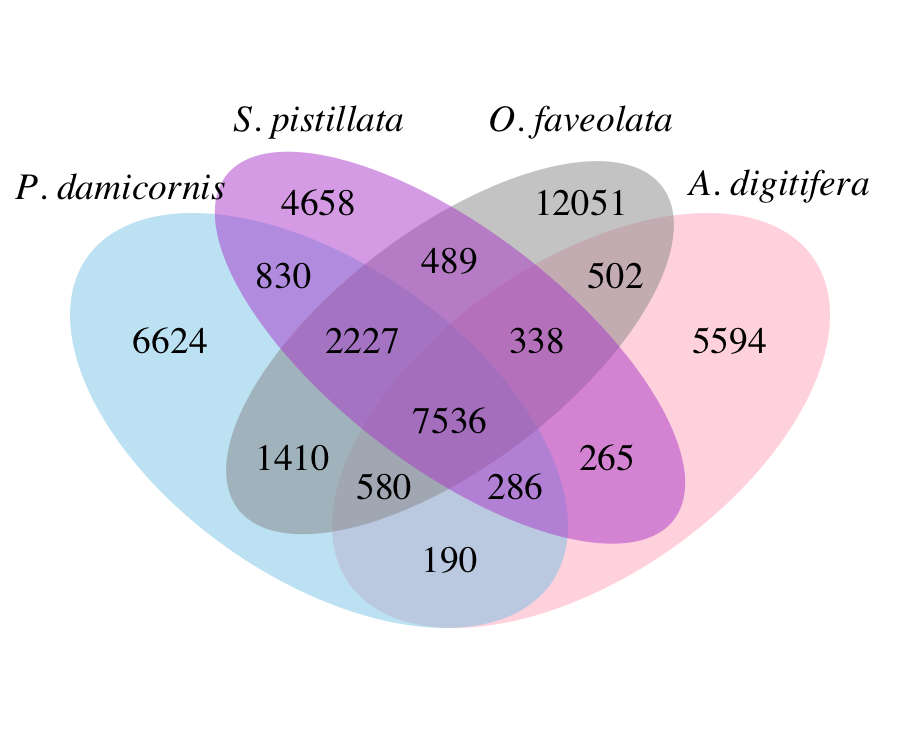
\includegraphics{../figures/coral_venn.png}
\caption{Figure 1a. Species-specific and shared gene families across
four scleractinian genomes. Numbers indicate the number of gene
families, which include both single-copy genes and multi-copy gene
families.}
\end{figure}

\begin{figure}
\centering
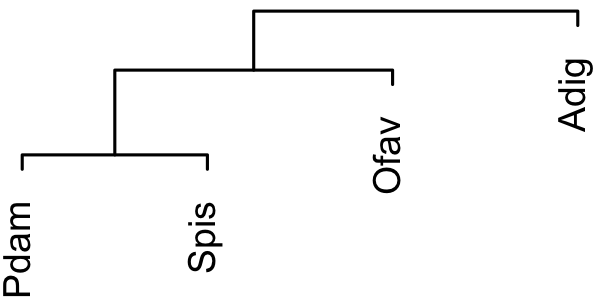
\includegraphics{../figures/coral_genecontent_dendro.png}
\caption{Figure 1b. Gene content dendrogram of four scleractinian
genomes.}
\end{figure}

\subsection{Coral core genes}\label{coral-core-genes}

The coral `core' gene families comprise 17.3\% of all gene families
identified among the four genomes. In \emph{P. damicornis}, core gene
family members totaled 12,147, or 46.6\% of all genes. Functional
profiling of this core genome in \emph{P. damicornis} revealed
significant enrichment of 44 GO terms associated with basic cellular
functions, including nucleic acid synthesis and processing, cellular
signaling and transport, and lipid, carbohydrate, and protein metabolism
(Fig. 2). This basic functionality explains why over 30\% of these gene
families are also found in all other cnidarians, and 96.3\% have
orthologs in at least one non-coral.

\begin{figure}
\centering
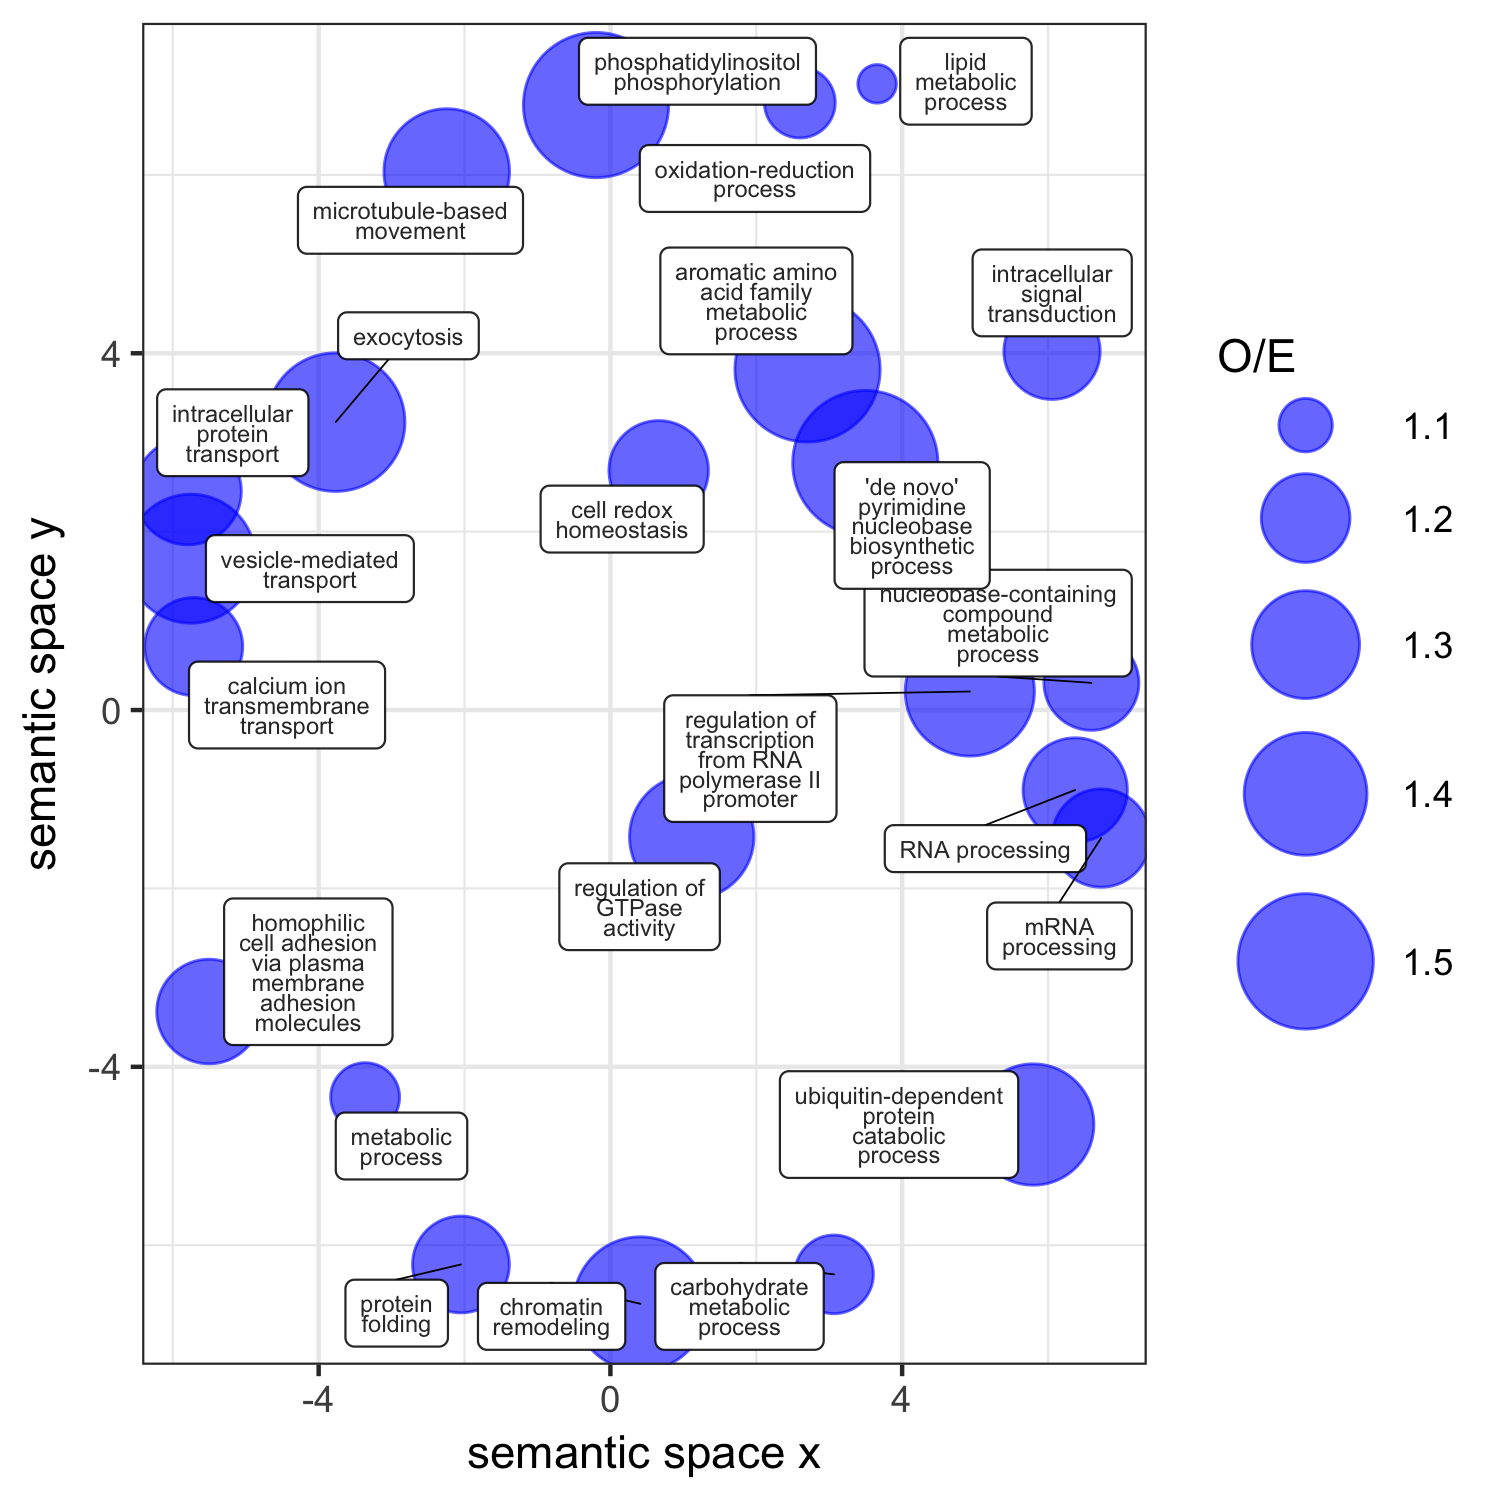
\includegraphics{../coral_core/coral_core_enriched_revigo.png}
\caption{Figure 2. Functional profile of the core coral genome in
\emph{P. damicornis}. Significantly enriched GO terms (p \textless{}
0.05) within this gene set were reduced (allowed similarity = 0.4) and
visualized in semantic space by REVIGO. Point size is scaled to the
ratio of observed to expected (O/E) occurrences of each GO term in the
coral core gene set.}
\end{figure}

\subsection{Coral-specific genes}\label{coral-specific-genes}

Among the coral core gene families, 278 (3.7\%) had no orthologs outside
Scleractinia, indicating these may be coral-specific gene families.
These coral-specific genes in \emph{P. damicornis} (n=349) showed
significant enrichment of GO terms related to immune function, such as
viral defense, signal transduction, and NF-\(\kappa\)B pathway
regulation (Fig. 3). The NF-\(\kappa\)B signaling pathway was
characterized as a key component of the innate immune response in
\emph{O. faveolata} (Williams et al. 2017). The 32 genes in this set
associated with signal transduction may also represent coral-specific
immune pathways; SwissProt annotations of these genes included dopamine
receptors, neuropeptide receptors, G-protein coupled receptors, and
tumor necrosis factor (TNF) receptor-associated factors (TRAFs). The TNF
receptor superfamily in \emph{A. digitifera}, comprised of 40 proteins,
is more diverse than any organism described thus far (Quistad et al.
2014; {\textbf{???}}), and these results suggest such genes and pathways
are broadly represented in corals. Indeed, \emph{P. damicornis}
contained 39 proteins with TNFR cysteine-rich domains. Finally, caveola
assembly, or the formation of structures in cell membranes that anchor
transmembrane proteins, may also serve an important role in signal
transduction and immunity (H. H. Patel and Insel 2009). Another enriched
function in the coral-specific gene set was copper ion transmembrane
transport, which may reflect an important role for delivery of copper to
endosymbionts, where it is a critical component of proteins involved in
photosynthesis (plastocyanin) and oxidative stress response (superoxide
dismutase) (Festa and Thiele 2011). Indeed, in mycorrhizal symbioses,
fungi deliver copper to the photosynthetic plant partner
(González-Guerrero et al. 2016). Other enriched functions in the
coral-specific genes include meiotic chromosome segregation, chromatin
silencing and regulation of transcription, and tetrahydrofolate
biosynthesis.

\begin{figure}
\centering
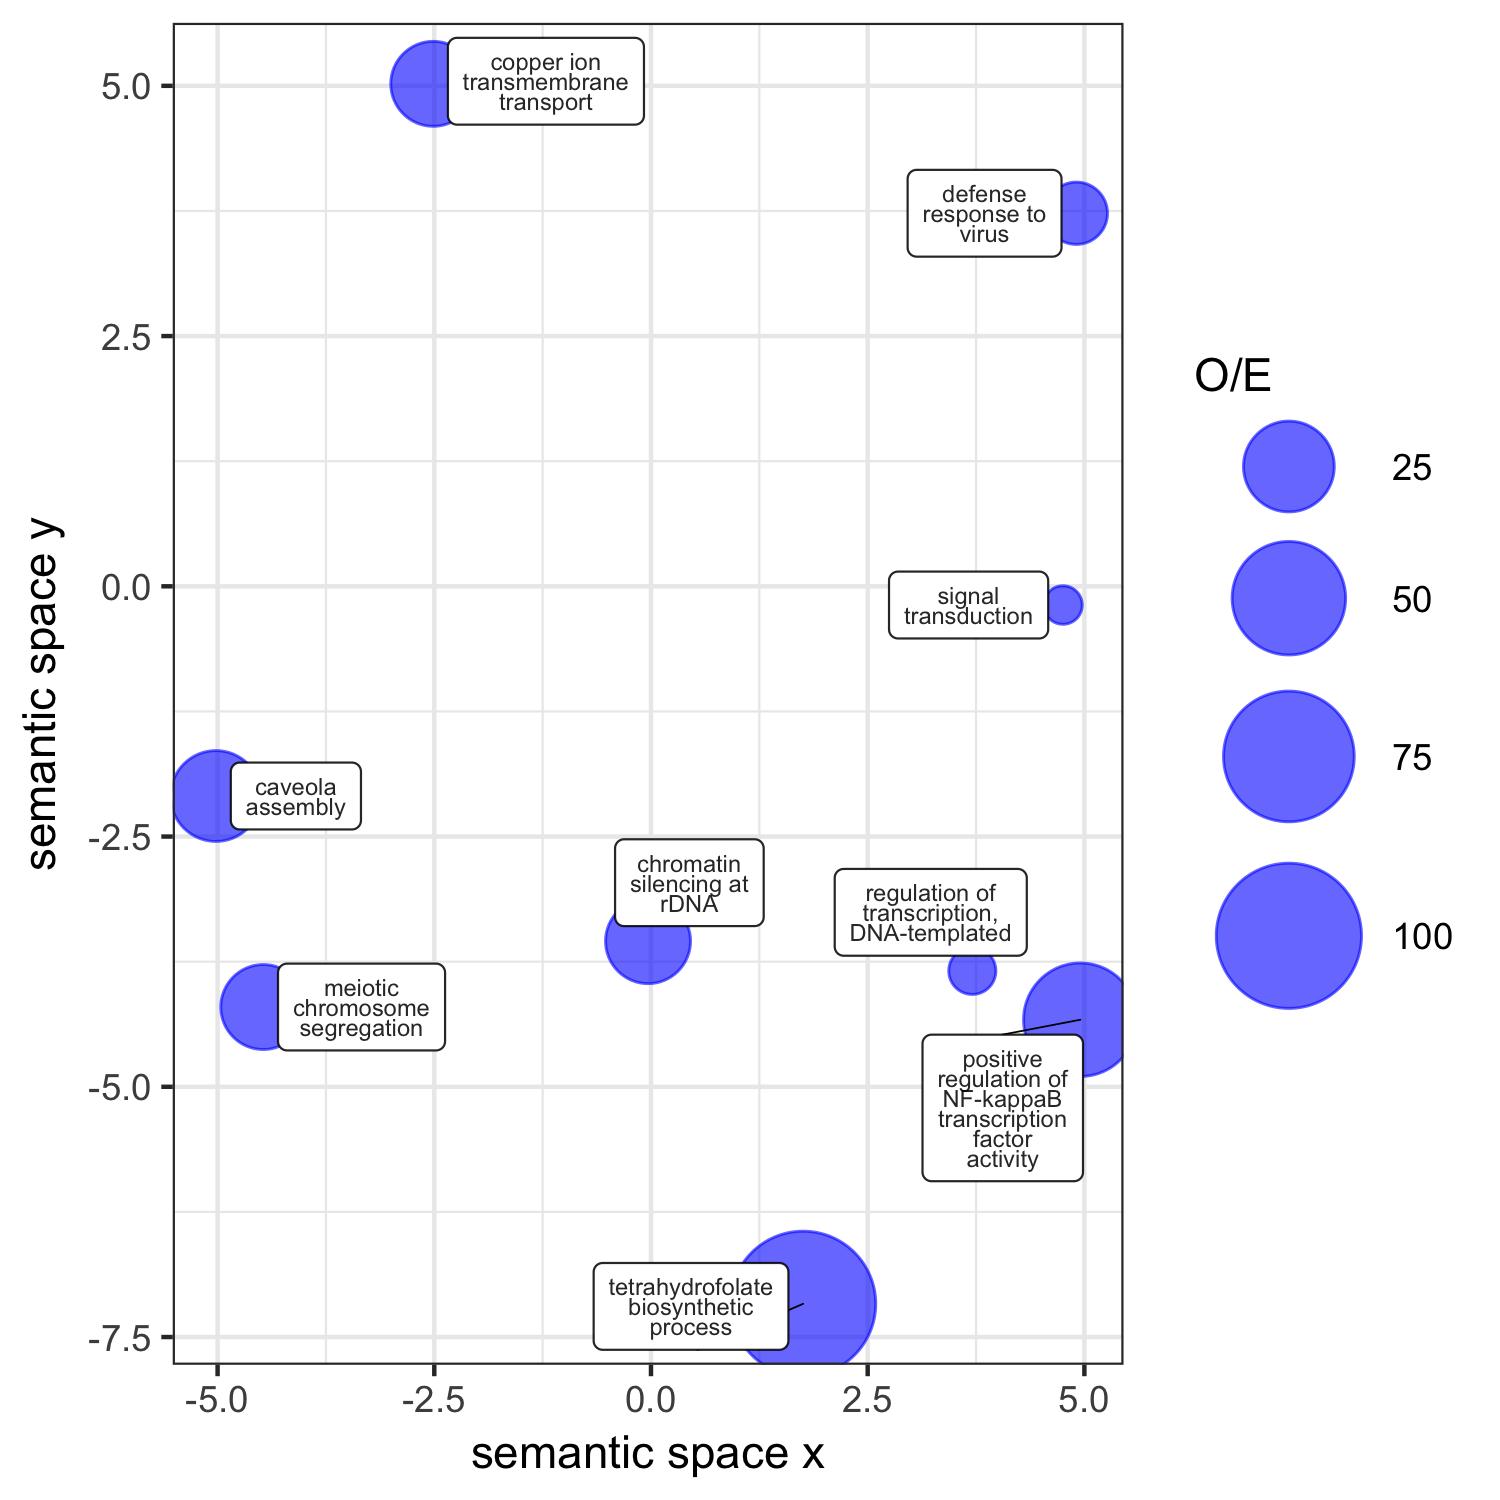
\includegraphics{../coral_specific/coral_specific_enriched_revigo.png}
\caption{Figure 3. Functional profile of coral-specific genes in
\emph{P. damicornis}. Significantly enriched GO terms (p \textless{}
0.05) within this gene set were reduced (allowed similarity = 0.7) and
visualized in semantic space by REVIGO. Point size is scaled to the
ratio of observed to expected (O/E) occurrences of each GO term in the
coral-specific gene set.}
\end{figure}

\subsection{Coral-diversified genes}\label{coral-diversified-genes}

Twenty-one gene families were diversified in corals, meaning that the
gene family was significantly larger in corals compared to corallimorphs
and anemones (\emph{p} \textless{} 0.01). Members of these
coral-diversified gene families in \emph{P. damicornis} (n=339) were
significantly enriched for 9 GO terms (Fig. 4) that suggest roles in
cellular signaling and possibly immunity. More detailed functional
annotation of representative genes from these 21 families was
accomplished by a BLAST search to the NCBI nr database (see
Supplementary Table SX), which revealed putative functionality with
links to key coral traits. Significant similarity was identified between
coral-diversified genes and proteins associated with apoptosis (e.g.,
tyrosine kinase and NFX1), stress response (e.g.~sacsin-like HSP70
co-chaperones), and ligand recognition and signaling (e.g., C-type
lectins, G-protein-coupled receptors), which may serve important roles
in coral symbiosis and immunity. Other coral-diversified genes were
similar to calcium ion channels (e.g., polycystins) and cell adhesion
proteins (e.g., hemicentins), which have been identified as components
of the skeletal organic matrix with important roles in biomineralization
(Ramos-Silva et al. 2013; Takeuchi et al. 2016)). We also found
significant similarities between coral-diversified genes and `euphy',
which accumulates as a yolk protein during coral oogenesis (Shikina et
al. 2015), and histone demethylase, which could indicate an important
role for epigenetic modifications that may underlie high levels of
phenotypic plasticity and aid in acclimatization to changing
environments. Interestingly, several annotations from this
coral-diversified gene set were also identified by R. A. Bay and Palumbi
(2014) corresponding to genes involved in heat resistance adaptation,
including E3 ubiquitin-protein ligase, tyrosine kinase, and hemicentin.

\begin{figure}
\centering
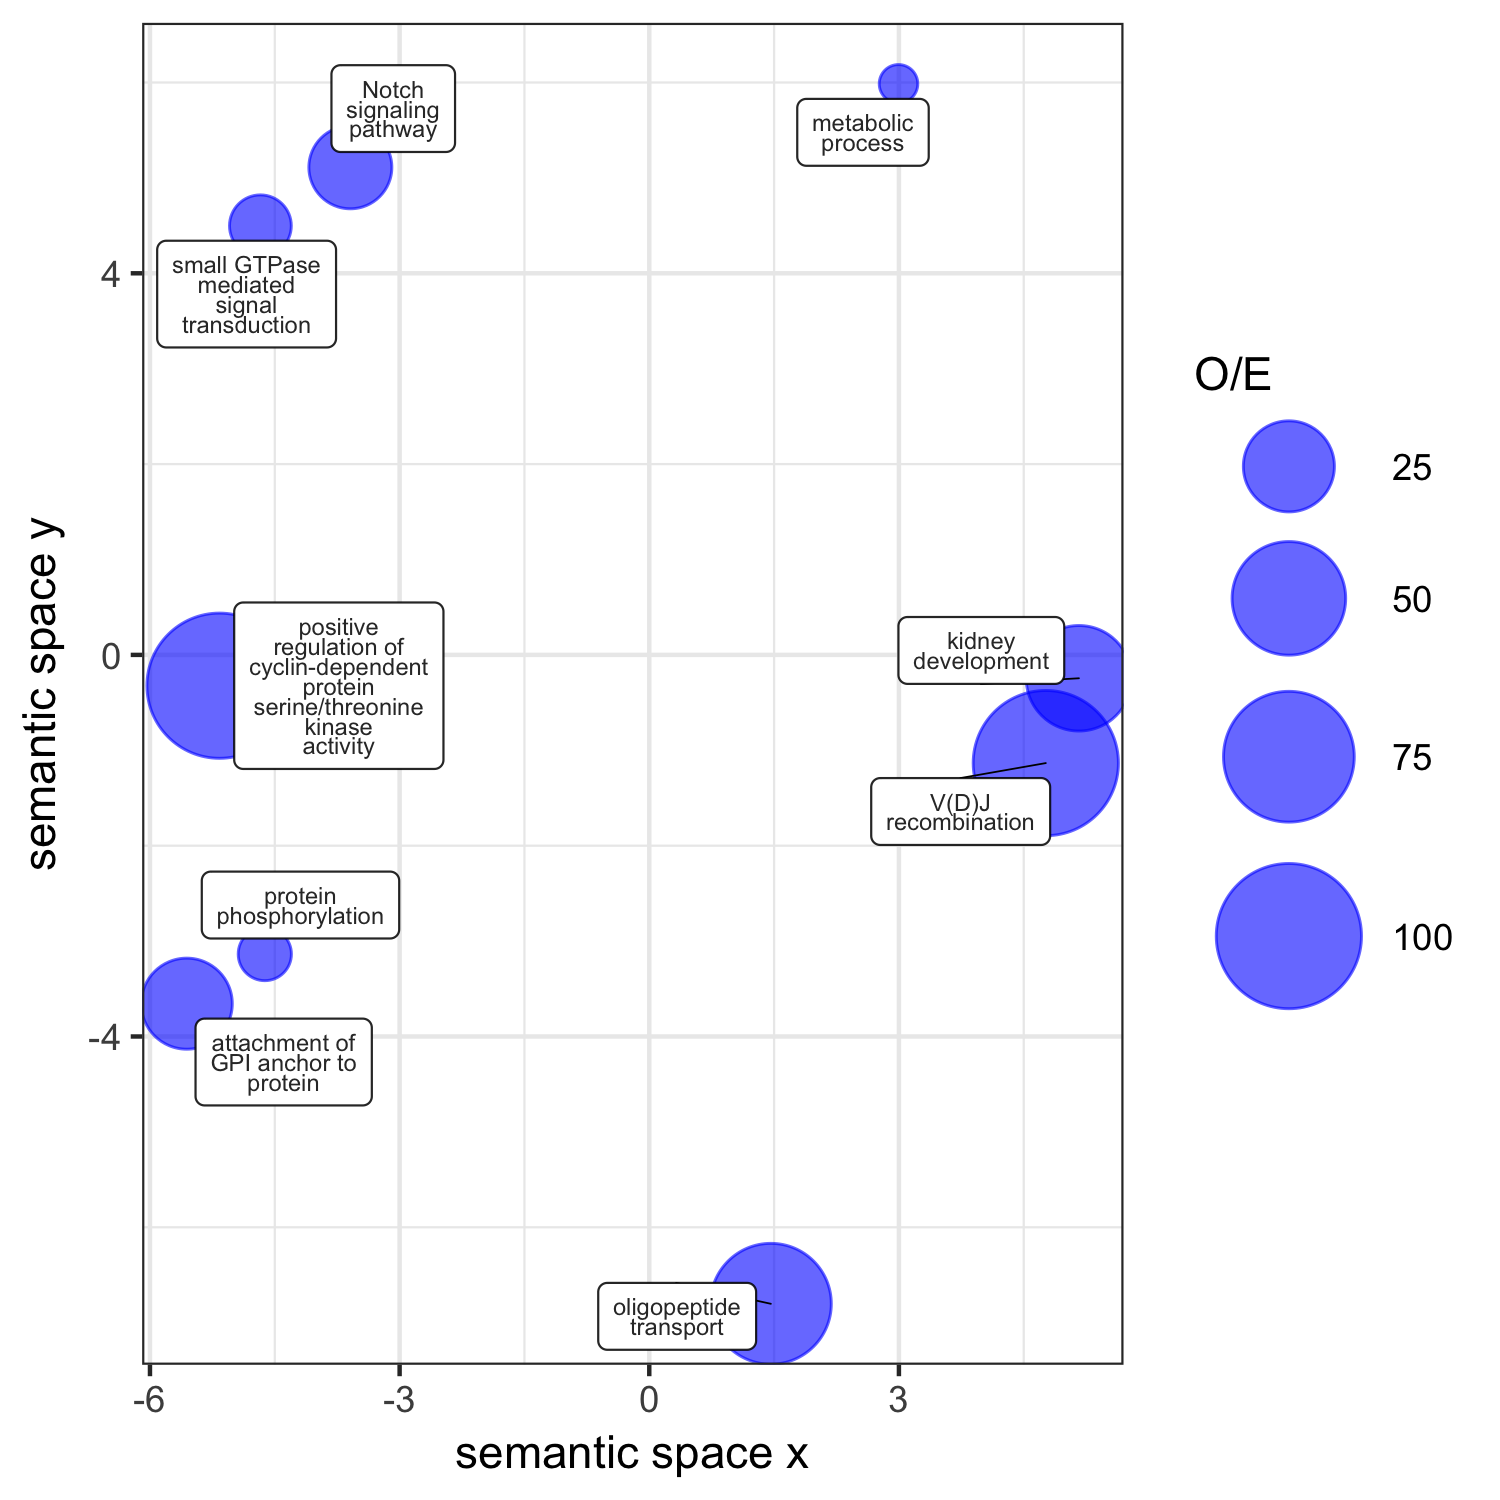
\includegraphics{../coral_diversified/coral_diversified_enriched_revigo.png}
\caption{Figure 4. Functional profile of coral-diversified genes in
\emph{P. damicornis}. Significantly enriched GO terms (p \textless{}
0.05) within this gene set were reduced (allowed similarity = 0.7) and
visualized in semantic space by REVIGO. Point size is scaled to the
ratio of observed to expected (O/E) occurrences of each GO term in the
coral-diversified gene set.}
\end{figure}

\subsection{Coral species-specific gene family
expansions}\label{coral-species-specific-gene-family-expansions}

The number of gene families in all corals decreased exponentially as
gene family size increased, consistent with patterns of gene family size
observed in other organisms {[}REFS{]} (Fig. 5). Interestingly, \emph{P.
damicornis} had the fewest large gene families (n=3 with
size\textgreater{}32, max size=75), and had smaller gene families
overall (Fig. 5). The largest gene families were observed in \emph{A.
digitifera} (n=25 with size\textgreater{}32, max size=255), consistent
with the comparative analysis of \emph{A. digitifera} and \emph{S.
pistillata} performed by (Voolstra et al. 2017). However, statistical
comparison of gene family sizes across the four coral species, which
accounts for differences in total genome size, indicated that \emph{S.
pistillata} had the most significantly expanded gene families relative
to other corals (n=15), followed by \emph{A. digitifera} (n=11).
\emph{O. faveolata} only had one gene family that was significantly
expanded, while \emph{P. damicornis} had none. (More here on
implications of different patterns of gene family expansion).

\begin{figure}
\centering
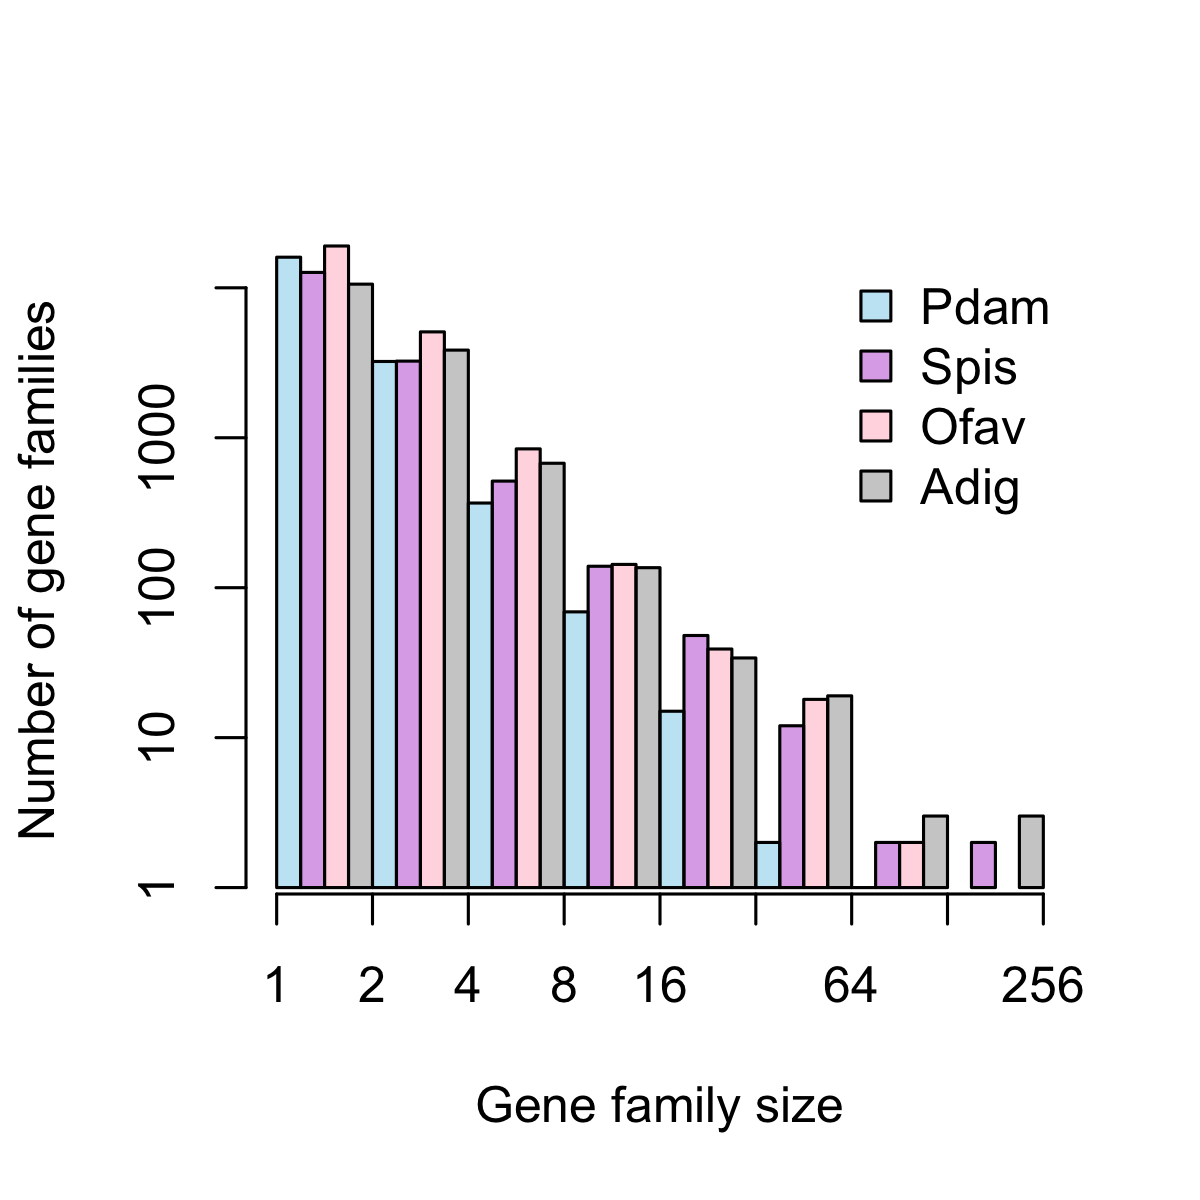
\includegraphics{../figures/gene_family_size.png}
\caption{Figure 5. Gene family size distribution in four coral genomes.}
\end{figure}

\subsection{\texorpdfstring{Uniqueness of \emph{P. damicornis}
genome}{Uniqueness of P. damicornis genome}}\label{uniqueness-of-p.-damicornis-genome}

\begin{itemize}
\tightlist
\item
  Smaller gene families
\item
  Fewer gene family expansions
\item
  Pdam-specific gene families
\end{itemize}

\subsection*{Conclusions}\label{conclusions}
\addcontentsline{toc}{subsection}{Conclusions}

\hypertarget{refs}{}
\hypertarget{ref-Alexa2016}{}
Alexa, Adrian, and Jorg Rahnenfuhrer. 2016. ``topGO: Enrichment Analysis
for Gene Ontology. R package version 2.24.0.''

\hypertarget{ref-Altschul1990}{}
Altschul, Stephen F, Warren Gish, Webb Miller, Eugene W Myers, and David
J Lipman. 1990. ``Basic local alignment search tool. - PubMed - NCBI.''
\emph{J. Mol. Biol.} 215 (3). National Center for Biotechnology
Information, National Library of Medicine, National Institutes of
Health, Bethesda, MD 20894.: 403--10.
\href{http://linkinghub.elsevier.com/retrieve/pii/S0022283605803602\%20papers3://publication/uuid/ABAD235C-2FD6-4AD7-8E80-8A6AA4054634}{http://linkinghub.elsevier.com/retrieve/pii/S0022283605803602 papers3://publication/uuid/ABAD235C-2FD6-4AD7-8E80-8A6AA4054634}.

\hypertarget{ref-Aranda2016}{}
Aranda, M, Y Li, Y J Liew, S Baumgarten, O Simakov, M C Wilson, J Piel,
et al. 2016. ``Genomes of coral dinoflagellate symbionts highlight
evolutionary adaptations conducive to a symbiotic lifestyle.''
\emph{Sci. Rep.} 6 (December). Nature Publishing Group: 39734.
\href{http://www.nature.com/srep/2016/161222/srep39734/full/srep39734.html\%20papers3://publication/doi/10.1038/srep39734}{http://www.nature.com/srep/2016/161222/srep39734/full/srep39734.html papers3://publication/doi/10.1038/srep39734}.

\hypertarget{ref-Baumgarten2015}{}
Baumgarten, Sebastian, Oleg Simakov, Lisl Y Esherick, Yi Jin Liew, Erik
M Lehnert, Craig T Michell, Yong Li, et al. 2015. ``The genome of
Aiptasia, a sea anemone model for coral symbiosis.'' \emph{PNAS},
August. National Acad Sciences, 201513318--62.
\href{http://www.pnas.org/lookup/doi/10.1073/pnas.1513318112\%20papers3://publication/doi/10.1073/pnas.1513318112}{http://www.pnas.org/lookup/doi/10.1073/pnas.1513318112 papers3://publication/doi/10.1073/pnas.1513318112}.

\hypertarget{ref-Bay2014}{}
Bay, Rachael A, and Stephen R Palumbi. 2014. ``Multilocus Adaptation
Associated with Heat Resistance in Reef-Building Corals.'' \emph{Curr.
Biol.} 24 (24). Department of Biology, Hopkins Marine Station of
Stanford University, Pacific Grove, CA 93950, USA. Electronic address:
rbay@stanford.edu.: Elsevier: 2952--6.
\href{http://www.cell.com/article/S0960982214013530/fulltext\%20papers3://publication/doi/10.1016/j.cub.2014.10.044}{http://www.cell.com/article/S0960982214013530/fulltext papers3://publication/doi/10.1016/j.cub.2014.10.044}.

\hypertarget{ref-Bay2017}{}
Bay, Rachael A, Noah H Rose, Cheryl A Logan, and Stephen R Palumbi.
2017. ``Genomic models predict successful coral adaptation if future
ocean warming rates are reduced,'' 1--10.
doi:\href{https://doi.org/10.1126/sciadv.1701413}{10.1126/sciadv.1701413}.

\hypertarget{ref-Bhattacharya2016}{}
Bhattacharya, Debashish, Shobhit Agrawal, Manuel Aranda, Sebastian
Baumgarten, Mahdi Belcaid, Jeana L Drake, Douglas Erwin, et al. 2016.
``Comparative genomics explains the evolutionary success of reef-forming
corals.'' \emph{Elife} 5 (May). Department of Ecology, Evolution;
Natural Resources, Rutgers University, New Brunswick, United States.:
eLife Sciences Publications Limited: e13288.
\href{http://elifesciences.org/lookup/doi/10.7554/eLife.13288\%20papers3://publication/doi/10.7554/eLife.13288}{http://elifesciences.org/lookup/doi/10.7554/eLife.13288 papers3://publication/doi/10.7554/eLife.13288}.

\hypertarget{ref-Campbell2014}{}
Campbell, Michael S, Carson Holt, Barry Moore, and Mark Yandell. 2014.
``Genome Annotation and Curation Using MAKER and MAKER-P.'' \emph{Curr.
Protoc. Bioinforma.} 48 (December). Eccles Institute of Human Genetics,
University of Utah, Salt Lake City, Utah.: John Wiley \& Sons, Inc.:
4.11.1--39.
\href{http://doi.wiley.com/10.1002/0471250953.bi0411s48\%20papers3://publication/doi/10.1002/0471250953.bi0411s48}{http://doi.wiley.com/10.1002/0471250953.bi0411s48 papers3://publication/doi/10.1002/0471250953.bi0411s48}.

\hypertarget{ref-Chapman2010}{}
Chapman, Jarrod a, Ewen F Kirkness, Oleg Simakov, Steven E Hampson,
Therese Mitros, Thomas Weinmaier, Thomas Rattei, et al. 2010. ``The
dynamic genome of Hydra.'' \emph{Nature} 464 (7288): 592--6.
doi:\href{https://doi.org/10.1038/nature08830}{10.1038/nature08830}.

\hypertarget{ref-Combosch2011}{}
Combosch, David J, and Steven V Vollmer. 2011. ``Population Genetics of
an Ecosystem-Defining Reef Coral Pocillopora damicornis in the Tropical
Eastern Pacific.'' \emph{PLoS One} 6 (8). Public Library of Science:
e21200.
\href{http://dx.plos.org/10.1371/journal.pone.0021200.pdf\%20papers3://publication/uuid/92329624-4E44-4C01-820E-28A202FF2C7F}{http://dx.plos.org/10.1371/journal.pone.0021200.pdf papers3://publication/uuid/92329624-4E44-4C01-820E-28A202FF2C7F}.

\hypertarget{ref-Costanza2014}{}
Costanza, R, R de Groot, and P Sutton. 2014. ``Changes in the global
value of ecosystem services.'' \emph{Glob. Environ. Chang.} 26
(January): 152--58.
\href{http://linkinghub.elsevier.com/retrieve/pii/S0959378014000685\%20papers3://publication/doi/10.1016/j.gloenvcha.2014.04.002}{http://linkinghub.elsevier.com/retrieve/pii/S0959378014000685 papers3://publication/doi/10.1016/j.gloenvcha.2014.04.002}.

\hypertarget{ref-Cunning_2013}{}
Cunning, Ross, and Andrew C Baker. 2013. ``Excess algal symbionts
increase the susceptibility of reef corals to bleaching.'' \emph{Nat.
Clim. Chang.} 3 (3). Nature Publishing Group: 259--62.
doi:\href{https://doi.org/10.1038/nclimate1711}{10.1038/nclimate1711}.

\hypertarget{ref-Dixon2015}{}
Dixon, Groves B, Sarah W Davies, Galina V Aglyamova, Eli Meyer, Line K
Bay, and Mikhail V Matz. 2015. ``Genomic determinants of coral heat
tolerance across latitudes.'' \emph{Science (80-. ).} 348 (6242).
Department of Integrative Biology, University of Texas at Austin, 205 W.
24th Street C0990, Austin, TX 78712, USA.: American Association for the
Advancement of Science: 1460--2.
doi:\href{https://doi.org/10.1126/science.1261224}{10.1126/science.1261224}.

\hypertarget{ref-Festa2011}{}
Festa, Richard A, and Dennis J Thiele. 2011. ``Copper: an Essential
Metal in Biology.'' \emph{Curr. Biol.} 21: R877--R883.
doi:\href{https://doi.org/10.1016/j.cub.2011.09.040}{10.1016/j.cub.2011.09.040}.

\hypertarget{ref-Finn2017}{}
Finn, Robert D, Teresa K Attwood, Patricia C Babbitt, Alex Bateman, Peer
Bork, Alan J Bridge, Hsin-Yu Chang, et al. 2017. ``InterPro in
2017---beyond protein family and domain annotations.'' \emph{Nucleic
Acids Res.} 45 (D1). Oxford University Press: D190--D199.
\href{https://academic.oup.com/nar/article-lookup/doi/10.1093/nar/gkw1107\%20papers3://publication/doi/10.1093/nar/gkw1107}{https://academic.oup.com/nar/article-lookup/doi/10.1093/nar/gkw1107 papers3://publication/doi/10.1093/nar/gkw1107}.

\hypertarget{ref-Fukami2008}{}
Fukami, H, A F Budd, A Collins, C C Wallace, Y-Y Chuang, Chaolun Allen
Chen, C-F Dai, K Iwao, Charles R C Sheppard, and Nancy Knowlton. 2008.
``Mitochondrial and nuclear genes suggest that stony corals are
monophyletic but most families of stony corals are not (Order
Scleractinia, Class anthozoa, phylum cnidaria).'' \emph{PLoS One} 3 (9).
Public Library of Science.
\href{http://www.scopus.com/scopus/record/display.url?fedsrfIntegrator=MEKPAPERS-SCOCIT\%7B/\&\%7Dorigin=fedsrf\%7B/\&\%7Dview=basic\%7B/\&\%7Deid=2-s2.0-52449129525\%20papers3://publication/uuid/73BB683C-0C57-45F2-B783-EA0E9877D7AD}{http://www.scopus.com/scopus/record/display.url?fedsrfIntegrator=MEKPAPERS-SCOCIT\{\textbackslash{}\&\}origin=fedsrf\{\textbackslash{}\&\}view=basic\{\textbackslash{}\&\}eid=2-s2.0-52449129525 papers3://publication/uuid/73BB683C-0C57-45F2-B783-EA0E9877D7AD}.

\hypertarget{ref-Glynn:2001p7571}{}
Glynn, Peter W, Juan L Maté, Andrew C Baker, and M O Calderón. 2001.
``Coral bleaching and mortality in Panama and Ecuador during the
1997-1998 El Ni\{ñ\}o-Southern Oscillation event: Spatial/temporal
patterns and comparisons with the 1982-1983 event.'' \emph{Bull. Mar.
Sci.} 69 (1): 79--109.

\hypertarget{ref-Gonzalez-Guerrero2016}{}
González-Guerrero, Manuel, Viviana Escudero, Ángela Saéz, and Manuel
Tejada-Jiménez. 2016. ``Transition Metal Transport in Plants and
Associated Endosymbionts: Arbuscular Mycorrhizal Fungi and Rhizobia.''
\emph{Front. Plant Sci.} 7 (July): 1--21.
doi:\href{https://doi.org/10.3389/fpls.2016.01088}{10.3389/fpls.2016.01088}.

\hypertarget{ref-Hall2014}{}
Hall, B., T. DeRego, and S. Geib. 2014. ``GAG: the Genome Annotation
Generator.''
\href{http://genomeannotation.github.io/GAG\%20papers3://publication/uuid/06EC7449-9A15-413F-B86E-005B3D486650}{http://genomeannotation.github.io/GAG papers3://publication/uuid/06EC7449-9A15-413F-B86E-005B3D486650}.

\hypertarget{ref-Johnston2017}{}
Johnston, Erika C., Zac H. Forsman, Jean-François Flot, Sebastian
Schmidt-Roach, Jorge H. Pinzón, Ingrid S. S. Knapp, and Robert J.
Toonen. 2017. ``A genomic glance through the fog of plasticity and
diversification in Pocillopora.'' \emph{Sci. Rep.} 7 (1): 5991.
doi:\href{https://doi.org/10.1038/s41598-017-06085-3}{10.1038/s41598-017-06085-3}.

\hypertarget{ref-Jokiel_1977}{}
Jokiel, P L, and S L Coles. 1977. ``Effects of temperature on the
mortality and growth of Hawaiian reef corals.'' \emph{Mar. Biol.} 43
(3). Springer Science \(\backslash\)mathplus Business Media: 201--8.
doi:\href{https://doi.org/10.1007/bf00402312}{10.1007/bf00402312}.

\hypertarget{ref-Jones2014a}{}
Jones, Philip, David Binns, Hsin Yu Chang, Matthew Fraser, Weizhong Li,
Craig McAnulla, Hamish McWilliam, et al. 2014. ``InterProScan 5:
Genome-scale protein function classification.'' \emph{Bioinformatics} 30
(9): 1236--40.
doi:\href{https://doi.org/10.1093/bioinformatics/btu031}{10.1093/bioinformatics/btu031}.

\hypertarget{ref-Kleypas1999}{}
Kleypas, Joan A, Robert W Buddemeier, D Archer, Jean-Pierre Gattuso,
Chris Langdon, and B N Opdyke. 1999. ``Geochemical consequences of
increased atmospheric carbon dioxide on coral reefs.'' \emph{Science
(80-. ).} 284 (5411). American Association for the Advancement of
Science: 118--20.
\href{http://www.scopus.com/inward/record.url?partnerID=yv4JPVwI\%7B/\&\%7Deid=2-s2.0-0033515744\%7B/\&\%7Dmd5=b8c037c7a3c204e96489f57f1a96fc1f\%20papers3://publication/uuid/0D610CB2-D4D7-4B62-9738-1B7E86C80E04}{http://www.scopus.com/inward/record.url?partnerID=yv4JPVwI\{\textbackslash{}\&\}eid=2-s2.0-0033515744\{\textbackslash{}\&\}md5=b8c037c7a3c204e96489f57f1a96fc1f papers3://publication/uuid/0D610CB2-D4D7-4B62-9738-1B7E86C80E04}.

\hypertarget{ref-Knowlton2010}{}
Knowlton, Nancy, Russell E. Brainard, Rebecca Fisher, Megan Moews,
Laetitia Plaisance, and M. Julian Caley. 2010. ``Coral Reef
Biodiversity.'' \emph{Life World's Ocean. Divers. Distrib. Abundance},
65--78.
doi:\href{https://doi.org/10.1002/9781444325508.ch4}{10.1002/9781444325508.ch4}.

\hypertarget{ref-McGinley_2012}{}
McGinley, M P, M D Aschaffenburg, D T Pettay, R T Smith, T C LaJeunesse,
and M E Warner. 2012. ``Symbiodinium spp. in colonies of eastern Pacific
Pocillopora spp. are highly stable despite the prevalence of
low-abundance background populations.'' \emph{Mar. Ecol. Prog. Ser.} 462
(August). Inter-Research Science Center: 1--7.
doi:\href{https://doi.org/10.3354/meps09914}{10.3354/meps09914}.

\hypertarget{ref-Neubauer2016a}{}
Neubauer, Emilie F., Angela Z. Poole, Virginia M. Weis, and Simon K.
Davy. 2016. ``The scavenger receptor repertoire in six cnidarian species
and its putative role in cnidarian-dinoflagellate symbiosis.''
\emph{PeerJ} 4: e2692.
doi:\href{https://doi.org/10.7717/peerj.2692}{10.7717/peerj.2692}.

\hypertarget{ref-van_Oppen_2015}{}
Oppen, Madeleine J H van, James K Oliver, Hollie M Putnam, and Ruth D
Gates. 2015. ``Building coral reef resilience through assisted
evolution.'' \emph{Proc. Natl. Acad. Sci.} 112 (8). Proceedings of the
National Academy of Sciences: 2307--13.
doi:\href{https://doi.org/10.1073/pnas.1422301112}{10.1073/pnas.1422301112}.

\hypertarget{ref-Patel2009}{}
Patel, Hemal H, and Paul A Insel. 2009. ``Lipid rafts and caveolae and
their role in compartmentation of redox signaling.'' \emph{Antioxid.
Redox Signal.} 11 (6): 1357--72.
doi:\href{https://doi.org/10.1089/ars.2008.2365}{10.1089/ars.2008.2365}.

\hypertarget{ref-Pinzon2011}{}
Pinzón, Jorge H, and Todd C LaJeunesse. 2011. ``Species delimitation of
common reef corals in the genus Pocillopora using nucleotide sequence
phylogenies, population genetics and symbiosis ecology.'' \emph{Mol.
Ecol.} 20 (January): 311--25.
\href{http://onlinelibrary.wiley.com/doi/10.1111/j.1365-294X.2010.04939.x/pdf\%20papers3://publication/uuid/EA7906B2-73F3-42B0-8CF7-4012B89FC86C}{http://onlinelibrary.wiley.com/doi/10.1111/j.1365-294X.2010.04939.x/pdf papers3://publication/uuid/EA7906B2-73F3-42B0-8CF7-4012B89FC86C}.

\hypertarget{ref-Pinzon2013}{}
Pinzón, Jorge H, Eugenia M Sampayo, Evelyn F Cox, Leonard J Chauka,
Chaolun Allen Chen, Christian R Voolstra, and Todd C LaJeunesse. 2013.
``Blind to morphology: genetics identifies several widespread
ecologically common species and few endemics among Indo-Pacific
cauliflower corals.'' Edited by Christine Maggs. \emph{J. Biogeogr.} 40
(8): 1--20.
\href{http://doi.wiley.com/10.1111/jbi.12110\%20papers3://publication/doi/10.1111/jbi.12110}{http://doi.wiley.com/10.1111/jbi.12110 papers3://publication/doi/10.1111/jbi.12110}.

\hypertarget{ref-Prada2016a}{}
Prada, Carlos, Bishoy Hanna, Ann F. Budd, Cheryl M. Woodley, Jeremy
Schmutz, Jane Grimwood, Roberto Iglesias-Prieto, et al. 2016. ``Empty
Niches after Extinctions Increase Population Sizes of Modern Corals.''
\emph{Curr. Biol.} 26 (23): 3190--4.
doi:\href{https://doi.org/10.1016/j.cub.2016.09.039}{10.1016/j.cub.2016.09.039}.

\hypertarget{ref-Putnam2016a}{}
Putnam, Nicholas H, Brendan L O'Connell, Jonathan C Stites, Brandon J
Rice, Marco Blanchette, Robert Calef, Christopher J Troll, et al. 2016.
``Chromosome-scale shotgun assembly using an in vitro method for
long-range linkage.'' \emph{Genome Res.} 26 (3). Dovetail Genomics LLC,
Santa Cruz, California 95060, USA; Cold Spring Harbor Laboratory Press:
342--50.
\href{http://genome.cshlp.org/lookup/doi/10.1101/gr.193474.115\%20papers3://publication/doi/10.1101/gr.193474.115}{http://genome.cshlp.org/lookup/doi/10.1101/gr.193474.115 papers3://publication/doi/10.1101/gr.193474.115}.

\hypertarget{ref-Putnam2007}{}
Putnam, Nicholas H, Mansi Srivastava, Uffe Hellsten, Bill Dirks, Jarrod
Chapman, Asaf Salamov, Astrid Terry, et al. 2007. ``Sea anemone genome
reveals ancestral eumetazoan gene repertoire and genomic organization.''
\emph{Science} 317 (5834): 86--94.
doi:\href{https://doi.org/10.1126/science.1139158}{10.1126/science.1139158}.

\hypertarget{ref-Quistad2014}{}
Quistad, Steven D., Aleksandr Stotland, Katie L. Barott, Cameron A.
Smurthwaite, Brett Jameson Hilton, Juris A. Grasis, Roland Wolkowicz,
and Forest L. Rohwer. 2014. ``Evolution of TNF-induced apoptosis reveals
550 My of functional conservation.'' \emph{Proc. Natl. Acad. Sci.} 111
(26). National Acad Sciences: 9567--72.
doi:\href{https://doi.org/10.1073/pnas.1405912111}{10.1073/pnas.1405912111}.

\hypertarget{ref-Ramos-Silva2013}{}
Ramos-Silva, Paula, Jaap Kaandorp, Lotte Huisman, Benjamin Marie,
Isabelle Zanella-Cl??on, Nathalie Guichard, David J. Miller, and
Fr??d??ric Marin. 2013. ``The skeletal proteome of the coral acropora
millepora: The evolution of calcification by co-option and domain
shuffling.'' \emph{Mol. Biol. Evol.} 30 (9): 2099--2112.
doi:\href{https://doi.org/10.1093/molbev/mst109}{10.1093/molbev/mst109}.

\hypertarget{ref-Ryan2013}{}
Ryan, J F, K Pang, C E Schnitzler, A D Nguyen, R T Moreland, D K
Simmons, B J Koch, et al. 2013. ``The genome of the ctenophore
Mnemiopsis leidyi and its implications for cell type evolution.''
\emph{Science (80-. ).} 342 (6164): 1242592.
doi:\href{https://doi.org/10.1126/science.1242592}{10.1126/science.1242592}.

\hypertarget{ref-Schmidt-Roach2014}{}
Schmidt-Roach, Sebastian, K J Miller, Petra Lundgren, and Nikos
Andreakis. 2014. ``With eyes wide open: a revision of species within and
closely related to the Pocillopora damicornis species complex
(Scleractinia; Pocilloporidae) using morphology \ldots{}.'' \emph{Zool.
J. Linn. Soc.}, January.
\href{http://onlinelibrary.wiley.com/doi/10.1111/zoj.12092/full\%20papers3://publication/uuid/FF435743-7FC4-4CB3-A64F-75A1885F1F1B}{http://onlinelibrary.wiley.com/doi/10.1111/zoj.12092/full papers3://publication/uuid/FF435743-7FC4-4CB3-A64F-75A1885F1F1B}.

\hypertarget{ref-Schmidt-Roach2012}{}
Schmidt-Roach, Sebastian, Karen J Miller, Erika Woolsey, Gabriele
Gerlach, and Andrew H Baird. 2012. ``Broadcast Spawning by Pocillopora
Species on the Great Barrier Reef.'' \emph{PLoS One} 7 (12). Public
Library of Science: e50847.
\href{http://www.plosone.org/article/info\%7B/\%\%7D3Adoi\%7B/\%\%7D2F10.1371\%7B/\%\%7D2Fjournal.pone.0050847\%20papers3://publication/doi/10.1371/journal.pone.0050847}{http://www.plosone.org/article/info\{\textbackslash{}\%\}3Adoi\{\textbackslash{}\%\}2F10.1371\{\textbackslash{}\%\}2Fjournal.pone.0050847 papers3://publication/doi/10.1371/journal.pone.0050847}.

\hypertarget{ref-Shikina2015}{}
Shikina, S., Y.-L. Chiu, Y.-H. Lee, and C.-F. Chang. 2015. ``From
Somatic Cells to Oocytes: A Novel Yolk Protein Produced by Ovarian
Somatic Cells in a Stony Coral, Euphyllia ancora.'' \emph{Biol. Reprod.}
93 (3): 57--57.
doi:\href{https://doi.org/10.1095/biolreprod.115.129643}{10.1095/biolreprod.115.129643}.

\hypertarget{ref-Shinzato2011}{}
Shinzato, Chuya, Eiichi Shoguchi, Takeshi Kawashima, Mayuko Hamada,
Kanako Hisata, Makiko Tanaka, Manabu Fujie, et al. 2011. ``Using the
Acropora digitifera genome to understand coral responses to
environmental change.'' \emph{Nature} 476 (7360). Marine Genomics Unit,
Okinawa Institute of Science; Technology Promotion Corporation, Onna,
Okinawa 904-0412, Japan.: Nature Publishing Group: 320--23.
\href{http://eutils.ncbi.nlm.nih.gov/entrez/eutils/elink.fcgi?dbfrom=pubmed\%7B/\&\%7Did=21785439\%7B/\&\%7Dretmode=ref\%7B/\&\%7Dcmd=prlinks\%20papers3://publication/doi/10.1038/nature10249}{http://eutils.ncbi.nlm.nih.gov/entrez/eutils/elink.fcgi?dbfrom=pubmed\{\textbackslash{}\&\}id=21785439\{\textbackslash{}\&\}retmode=ref\{\textbackslash{}\&\}cmd=prlinks papers3://publication/doi/10.1038/nature10249}.

\hypertarget{ref-Shoguchi2013}{}
Shoguchi, Eiichi, Chuya Shinzato, Takeshi Kawashima, Fuki Gyoja, Sutada
Mungpakdee, Ryo Koyanagi, Takeshi Takeuchi, et al. 2013. ``Draft
Assembly of the Symbiodinium minutum Nuclear Genome Reveals
Dinoflagellate Gene Structure.'' \emph{Curr. Biol.} 23 (15). Elsevier:
1399--1408.
\href{http://dx.doi.org/10.1016/j.cub.2013.05.062\%20papers3://publication/doi/10.1016/j.cub.2013.05.062}{http://dx.doi.org/10.1016/j.cub.2013.05.062 papers3://publication/doi/10.1016/j.cub.2013.05.062}.

\hypertarget{ref-Simao2015}{}
Simão, Felipe A, Robert M Waterhouse, Panagiotis Ioannidis, Evgenia V
Kriventseva, and Evgeny M Zdobnov. 2015. ``BUSCO: assessing genome
assembly and annotation completeness with single-copy orthologs.''
\emph{Bioinformatics} 31 (19). Oxford University Press: 3210--2.
\href{https://academic.oup.com/bioinformatics/article-lookup/doi/10.1093/bioinformatics/btv351\%20papers3://publication/doi/10.1093/bioinformatics/btv351}{https://academic.oup.com/bioinformatics/article-lookup/doi/10.1093/bioinformatics/btv351 papers3://publication/doi/10.1093/bioinformatics/btv351}.

\hypertarget{ref-Snel1999}{}
Snel, B, P Bork, and M a Huynen. 1999. ``Genome phylogeny based on gene
content.'' \emph{Nat. Genet.} 21 (1): 108--10.
doi:\href{https://doi.org/10.1038/5052}{10.1038/5052}.

\hypertarget{ref-Srivastava2010}{}
Srivastava, Mansi, Oleg Simakov, Jarrod Chapman, Bryony Fahey, Marie E A
Gauthier, Therese Mitros, Gemma S Richards, et al. 2010. ``The
Amphimedon queenslandica genome and the evolution of animal
complexity.'' \emph{Nature} 466 (7307). Nature Publishing Group:
720--26.
doi:\href{https://doi.org/10.1038/nature09201}{10.1038/nature09201}.

\hypertarget{ref-Stanke2004}{}
Stanke, M, R Steinkamp, S Waack, and B Morgenstern. 2004. ``AUGUSTUS: a
web server for gene finding in eukaryotes.'' \emph{Nucleic Acids Res.}
32 (Web Server issue). University of Göttingen, Institut für
Mikrobiologie und Genetik, Goldschmidtstrasse 1, 37077 Göttingen,
Germany. mstanke@gwdg.de: Oxford University Press: W309--W312.
\href{https://academic.oup.com/nar/article-lookup/doi/10.1093/nar/gkh379\%20papers3://publication/doi/10.1093/nar/gkh379}{https://academic.oup.com/nar/article-lookup/doi/10.1093/nar/gkh379 papers3://publication/doi/10.1093/nar/gkh379}.

\hypertarget{ref-Stoddart1984}{}
Stoddart, J a. 1984. ``Genetical structure within populations of the
corals Pocillopora damicornis.'' \emph{Mar. Biol.} 81: 19--30.

\hypertarget{ref-Stoddart1983}{}
Stoddart, J. A. 1983. ``Asexual production of planulae in the coral
Pocillopora damicornis.'' \emph{Mar. Biol.} 76 (3): 279--84.
doi:\href{https://doi.org/10.1007/BF00393029}{10.1007/BF00393029}.

\hypertarget{ref-Supek2011}{}
Supek, Fran, Matko Bošnjak, Nives Škunca, and Tomislav Šmuc. 2011.
``Revigo summarizes and visualizes long lists of gene ontology terms.''
\emph{PLoS One} 6 (7).
doi:\href{https://doi.org/10.1371/journal.pone.0021800}{10.1371/journal.pone.0021800}.

\hypertarget{ref-Takeuchi2016}{}
Takeuchi, Takeshi, Lixy Yamada, Chuya Shinzato, Hitoshi Sawada, and
Noriyuki Satoh. 2016. ``Stepwise evolution of coral biomineralization
revealed with genome-wide proteomics and transcriptomics.'' \emph{PLoS
One} 11 (6).
doi:\href{https://doi.org/10.1371/journal.pone.0156424}{10.1371/journal.pone.0156424}.

\hypertarget{ref-TheUniProtConsortium2017}{}
The~UniProt~Consortium. 2017. ``UniProt: the universal protein
knowledgebase.'' \emph{Nucleic Acids Res.} 45 (D1). Oxford University
Press: D158--D169.
\href{https://academic.oup.com/nar/article-lookup/doi/10.1093/nar/gkw1099\%20papers3://publication/doi/10.1093/nar/gkw1099}{https://academic.oup.com/nar/article-lookup/doi/10.1093/nar/gkw1099 papers3://publication/doi/10.1093/nar/gkw1099}.

\hypertarget{ref-Thomas2017}{}
Thomas, Luke, W. Jason Kennington, Richard D. Evans, Gary A. Kendrick,
and Michael Stat. 2017. ``Restricted gene flow and local adaptation
highlight the vulnerability of high-latitude reefs to rapid
environmental change.'' \emph{Glob. Chang. Biol.} 23 (6): 2197--2205.
doi:\href{https://doi.org/10.1111/gcb.13639}{10.1111/gcb.13639}.

\hypertarget{ref-Voolstra2017}{}
Voolstra, Christian R, Yong Li, Yi Jin Liew, and Sebastian Baumgarten.
2017. ``Comparative analysis of the genomes of Stylophora pistillata and
Acropora digitifera provides evidence for extensive differences between
species of corals.''

\hypertarget{ref-Wang2017a}{}
Wang, Xin, Yi Jin Liew, Yong Li, Didier Zoccola, Sylvie Tambutte, and
Manuel Aranda. 2017. ``Draft genomes of the corallimorpharians
Amplexidiscus fenestrafer and Discosoma sp.'' \emph{Mol. Ecol. Resour.}
2017 (March): doi: 10.1111/1755--0998.12680.
doi:\href{https://doi.org/10.1111/1755-0998.12680}{10.1111/1755-0998.12680}.

\hypertarget{ref-Ward1992}{}
Ward, S. 1992. ``Evidence for broadcast spawning as well as brooding in
the scleractinian coral Pocillopora damicornis.'' \emph{Mar. Biol.} 112
(4): 641--46.
doi:\href{https://doi.org/10.1007/BF00346182}{10.1007/BF00346182}.

\hypertarget{ref-Williams2017}{}
Williams, Leah M., Lauren E. Fuess, Joseph J. Brennan, Katelyn M.
Mansfield, Erick Salas-Rodriguez, Julianne Welsh, Jake Awtry, et al.
2017. ``A conserved toll-like receptor-to-NF-\(\kappa\)B signaling
pathway in the endangered coral Orbicella faveolata.'' \emph{Dev. Comp.
Immunol.} Elsevier Ltd.
doi:\href{https://doi.org/10.1016/j.dci.2017.10.016}{10.1016/j.dci.2017.10.016}.

\end{document}


